
% Asset ID: A21RadiansTikZ-005
% Purpose: Show segment area as sector area minus triangle area.
\documentclass[tikz,border=8pt]{standalone}
\usetikzlibrary{angles,quotes}
\begin{document}
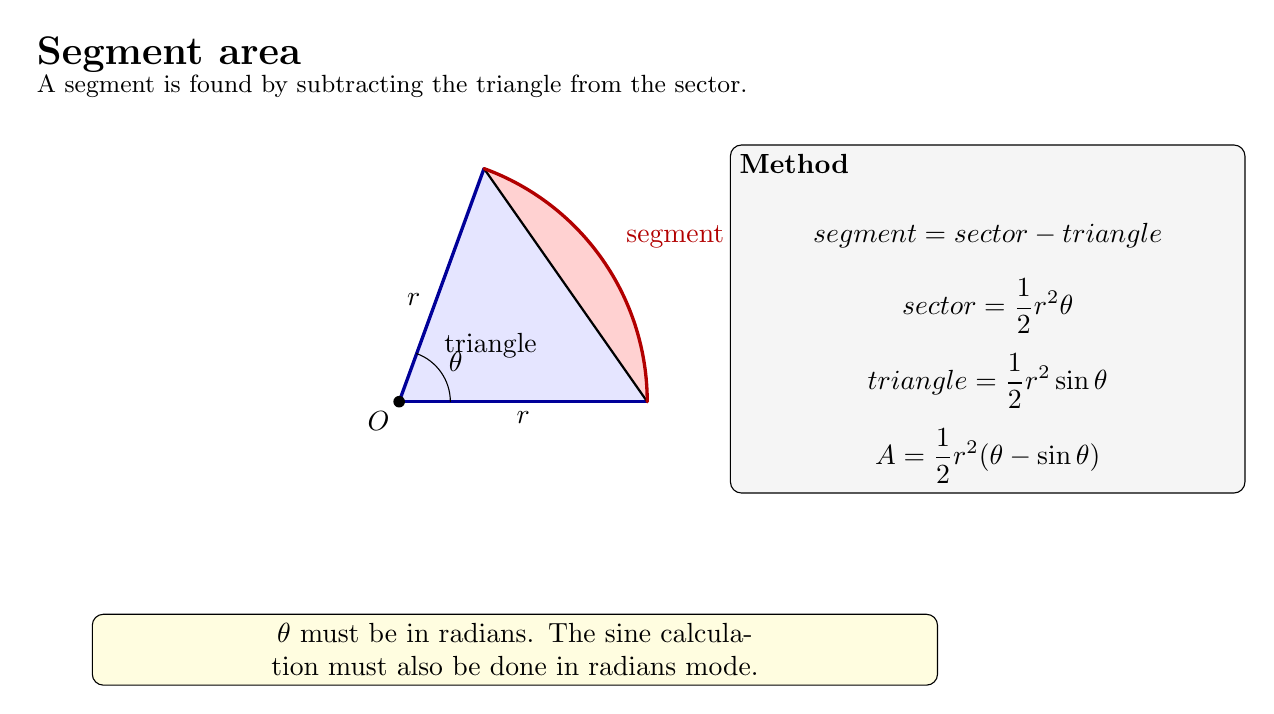
\begin{tikzpicture}[scale=1.05,line cap=round,line join=round]
\def\r{3}\def\ang{70}
\node[anchor=west,font=\bfseries\Large] at (-4.5,4.2) {Segment area};
\node[anchor=west,font=\small] at (-4.5,3.82) {A segment is found by subtracting the triangle from the sector.};
\coordinate (O) at (0,0);\coordinate (A) at (\r,0);\coordinate (B) at ({\r*cos(\ang)},{\r*sin(\ang)});
\fill[blue!10] (O)--(A) arc[start angle=0,end angle=\ang,radius=\r]--cycle;\fill[red!18] (A) arc[start angle=0,end angle=\ang,radius=\r]--cycle;
\draw[blue!60!black,very thick] (O)--(A);\draw[blue!60!black,very thick] (O)--(B);\draw[black,thick] (A)--(B);\draw[red!70!black,very thick] (A) arc[start angle=0,end angle=\ang,radius=\r];
\pic[draw=black,angle radius=0.65cm,angle eccentricity=1.35,"\(\theta\)"] {angle=A--O--B};
\fill (O) circle (2pt) node[below left] {\(O\)};\node[below] at (1.5,0) {\(r\)};\node[left] at ({1.1*cos(\ang)},{1.1*sin(\ang)+0.2}) {\(r\)};\node[right,red!70!black] at ({2.6*cos(35)+0.5},{2.6*sin(35)+0.5}) {segment};\node at ({1.35*cos(35)},{1.35*sin(35)-0.1}) {triangle};
\node[draw,rounded corners,fill=gray!8,anchor=west,align=left,text width=6.3cm] at (4.0,1.0) {\textbf{Method}\\[3pt]\[\text{segment}=\text{sector}-\text{triangle}\]\[\text{sector}=\frac12r^2\theta\]\[\text{triangle}=\frac12r^2\sin\theta\]\[\boxed{A=\frac12r^2(\theta-\sin\theta)}\]};
\node[draw,rounded corners,fill=yellow!12,align=center,text width=10.5cm] at (1.4,-3.0) {\(\theta\) must be in radians. The sine calculation must also be done in radians mode.};
\end{tikzpicture}
\end{document}
